\section{Results}
\label{sec:results}

\subsection{Datasets}
We evaluated our algorithms on three publicly available datasets. The first is the MNE sample dataset~\citep{gramfort2013meg} containing 204 gradiometer sensors (1 globally bad) and 102 magnetometer sensors. The second is the EEGBCI motor dataset~\citep{goldberger2000physiobank} with 104 subjects and the final one is the Faces dataset~\citep{wakeman2015multi} with 19 subjects. The bad channel annotations for each run and subject was available from the authors of the Faces dataset~\citep{wakeman2015multi}.

For the EEGBCI and MNE sample dataset, the trials are 700 ms long with a baseline period of 200 ms with respect to the trigger (auditory left tone for MNE sample and resting for EEGBCI). In the Faces dataset, we use the trials where famous faces were shown. The data was bandpass filtered between 1 and 40 Hz. The trials were 1 s long with a baseline period of 200 ms. 

\subsection{Auto reject (global)}

\begin{figure}[t!]
	\begin{center}
	\includegraphics[width=0.6\linewidth]{figures/figure4.pdf}
    \end{center}
    \caption{The evoked response (average of data across trials) on the sample dataset (Section~\ref{sec:results}) for gradiometer sensors before and after applying the \emph{auto reject} algorithm. Each sensor is a curve on the plots. Manually annotated bad sensor is shown in red. The algorithm finds the bad sensor automatically and repairs it for the relevant trials.
%     XXX here it is a bit better, could be more emphasized. % mj: cool
    }
    \label{fig:evoked}
\end{figure}

% this will be a problem, we don't have necessarily a permission for this. Needs to be fixed.
% XXX general remark: the figures are juxtaposed, it is correct that the interpretatio is postponed but you should summarize what can be seen there. Also make sure you use simple past for reporting results VS simple present general rules, basic report language 

Figure~\ref{fig:basic_cv} shows how the global threshold can be selected by cross-validation. One can observe how a low rejection threshold leads to high RMSE due to removal of too many trials whereas high rejection threshold leads to high RMSE because the bad trials are not removed. The reader may note that the automatic threshold is very close to a carefully chosen manual threshold. Figure~\ref{fig:hist}A shows the results computed for 104 subjects in the EEGBCI dataset. Note that the threshold does indeed vary across subjects.

\subsection{Auto reject (local)}

\begin{figure}[t]
	\begin{center}
	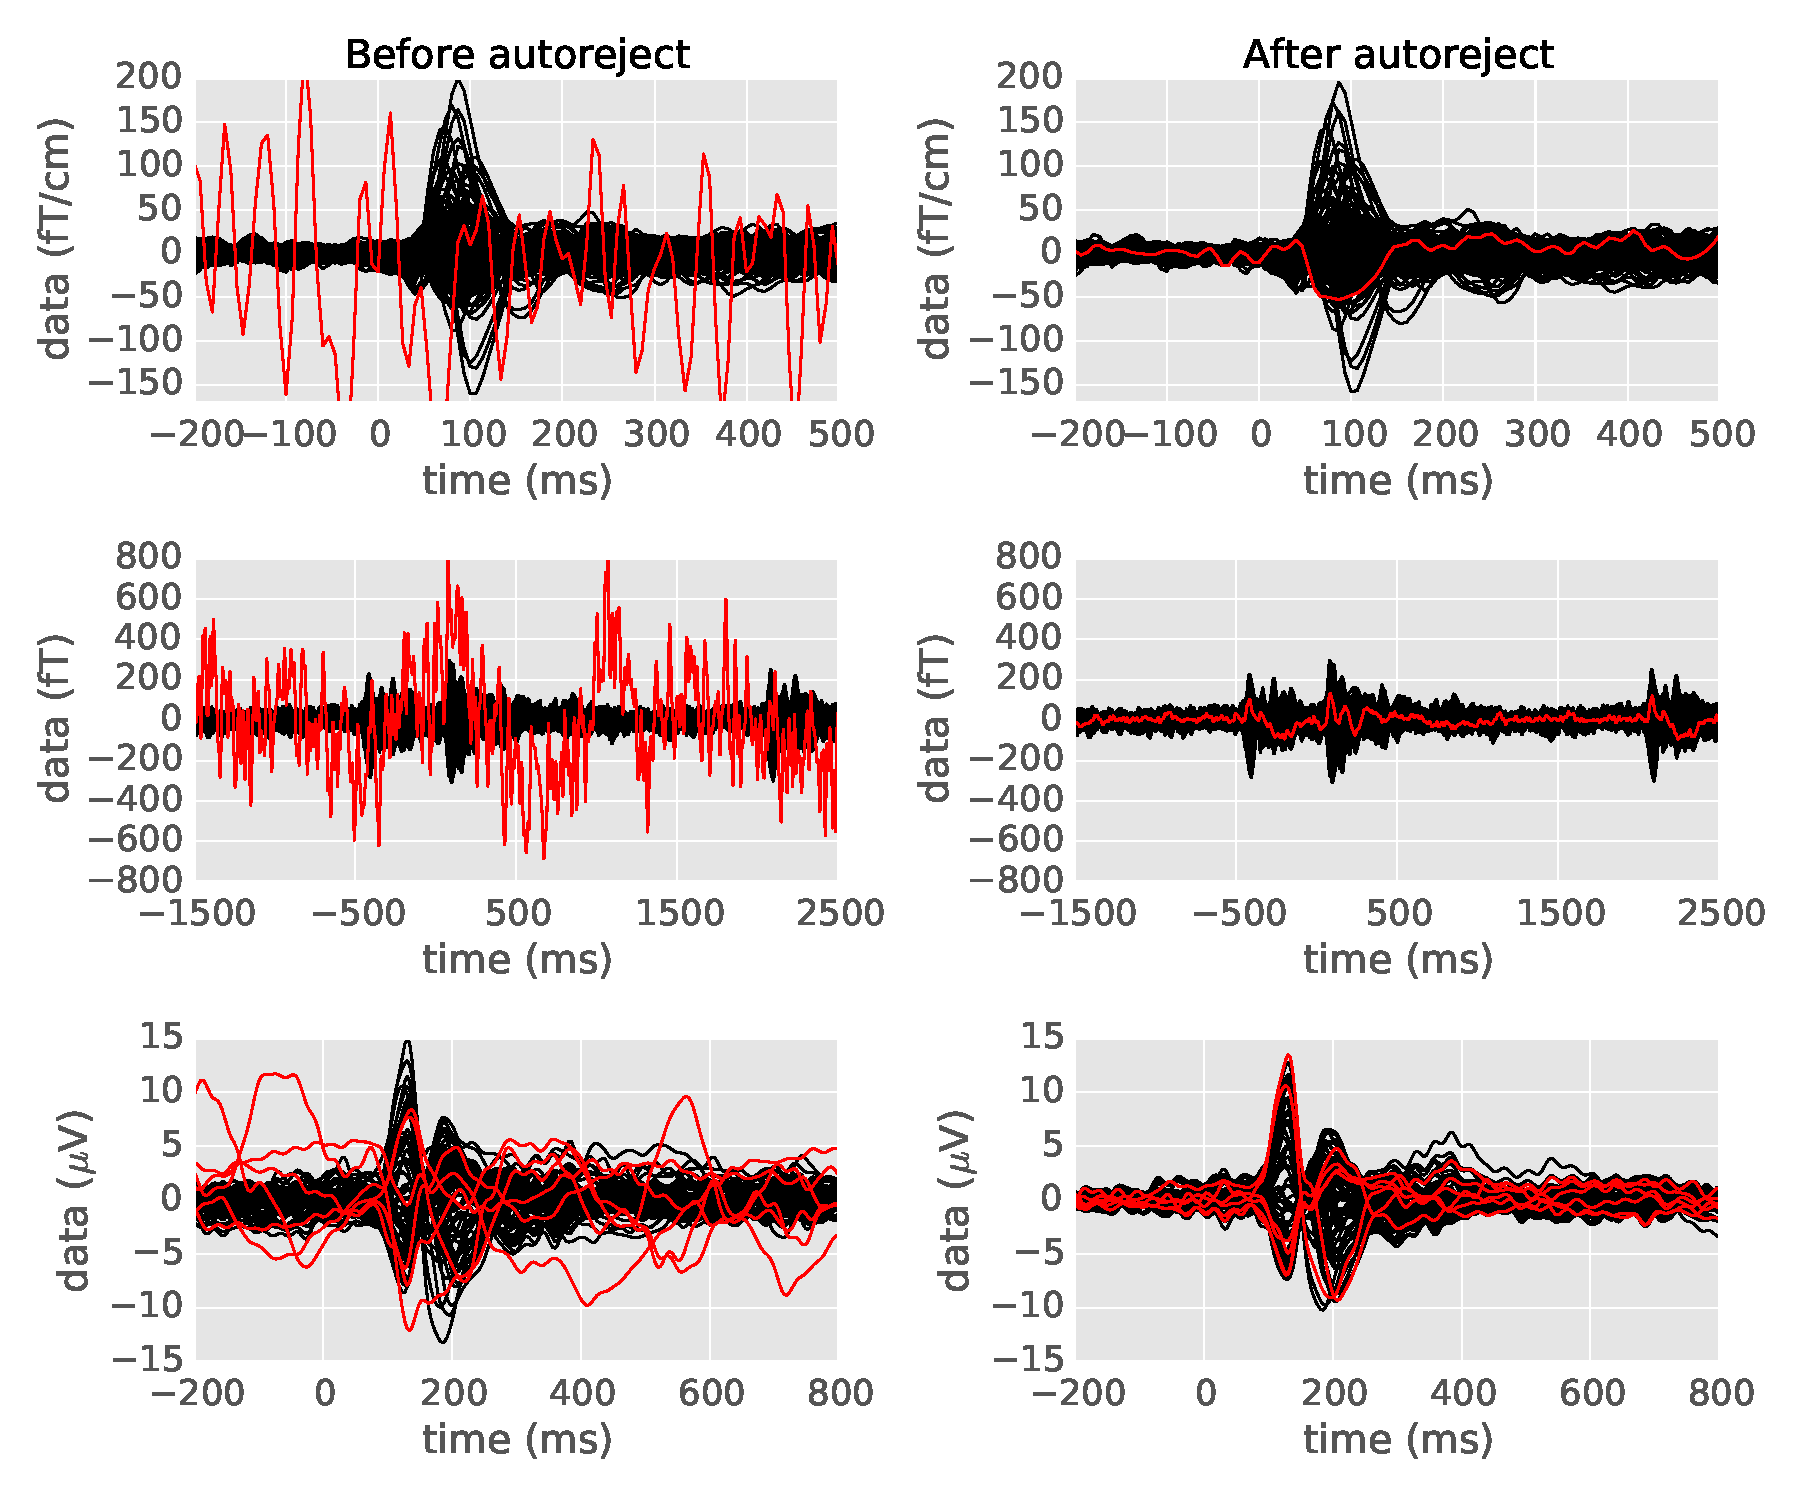
\includegraphics[width=0.7\linewidth]{figures/figure5.pdf}
    \end{center}
    \caption{RMSE with no rejection applied, \emph{auto reject (global)}, and RANSAC. Each point represents a subject from the Faces dataset \citep{wakeman2015multi}. \emph{Auto reject} has a better RMSE whenever a point lies above the dotted red line. Note that \emph{auto reject} almost always performs as well as or better than the other methods.}
    \label{fig:rmse_comparison}
\end{figure}

This auto reject (local) approach finds the thresholds at the level of each sensor. The candidate thresholds used vary between 2--400 $\mu V$ for EEG; 400--20000 fT/cm for gradiometers; and 400--20000 fT for magnetometers.

Figure~\ref{fig:hist}B demonstrates that the sensor-level thresholds for rejection are indeed different across sensors. This is the motivation for the more fine-grained technique based on consensus. \iftoggle{long}{Figure~\ref{fig:fine_reject} shows how the cross-validation curve varies with the consensus percentage and the maximum number of sensors which can be interpolated. Note how increasing both the parameters too much will in fact result in a worse RMSE. This is the reason why $\rho$ and $\kappa$ must be optimized jointly using grid search.}{} Figure~\ref{fig:evoked} demonstrates that the algorithm indeed improves the data quality. The bad MEG sensor which showed high fluctuations before applying the algorithm is repaired after application of the algorithm.

We compared our proposed algorithm to the RANSAC implementation in the PREP pipeline~\citep{bigdely2015prep}. RANSAC being an algorithm robust to outliers, serves as a competitive benchmark. To generate the ground truth for comparison, 4/5ths of the available trials were averaged and the bad channels interpolated per run. Outliers will have negligible effect in the ground-truth as it is obtained by averaging a large number of trials. It is this ground-truth which is used for computing the RMSE. This is a nested cross-validation setting where the validation set used for optimizing the thresholds is different from the ground truth (test set). The bad sensors detected by RANSAC (with default parameters) were interpolated before comparison to the ground truth. Figure~\ref{fig:rmse_comparison} shows that \emph{auto reject (local)} indeed does better than not rejecting trials or applying RANSAC. Of course, if  annotations of bad sensors per epochs were available, \emph{auto reject} will have an even better score because of how it works. We found that RANSAC results depend greatly on the input parameters which is probably why it does not perform as well as \emph{auto reject}.
